\documentclass{standalone}
\usepackage{tikz}
\usepackage[colorlinks=true]{hyperref}
\usetikzlibrary{
  arrows,
  calc,
  decorations.pathmorphing,
  decorations.pathreplacing,
  decorations.markings,
  positioning,
  shapes,
  arrows.meta
}
\tikzset{
  mid arrow/.style={postaction={decorate,decoration={
        markings,
        mark=at position .5 with {\arrow[#1]{stealth}}
      }}},
  mid arrow2/.style={postaction={decorate,decoration={
        markings,
        mark=at position .5 with {\arrow[>=stealth]{><}}
      }}},
}

\newcommand\drawlens[3]{
  % 1: center (x, y)
  % 2: size
  % 3: angle
  \begin{scope}[shift={#1}]
    \node[rotate={#3}] at (0, 0) {\scalebox{#2}{
\includegraphics[width=2cm]{fadings/lens.png}}};
  \end{scope}
}
\newcommand\drawwaveplate[3]{
  % 1: center (x, y)
  % 2: size
  % 3: angle
  \begin{scope}[shift={#1}]
    \node[rotate={#3}] at (0, 0)
    {\scalebox{#2}{
\includegraphics[width=2cm]{fadings/waveplate.png}}};
  \end{scope}
}
\newcommand\drawaom[4]{
  % 1: center (x, y)
  % 2: xsize
  % 3: ysize
  % 4: angle
  \begin{scope}[shift={#1}]
    \node[rotate={#4}] at (0, 0)
    {\scalebox{#2}[#3]{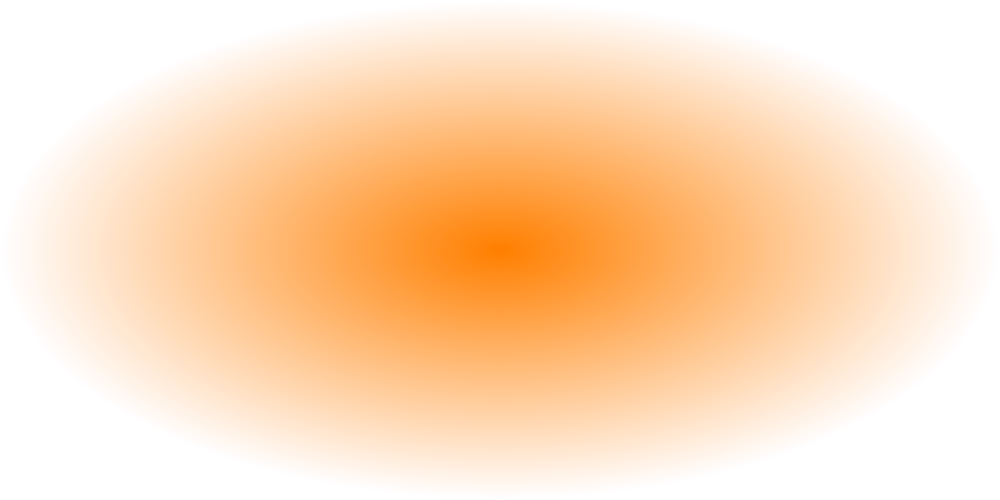
\includegraphics[width=2cm,height=2cm]{fadings/aom.png}}};
  \end{scope}
  \begin{scope}[rotate around={#4:#1}]
    \fill[orange, even odd rule, opacity=0.8]
    ($#1 + ({#2}, 0)$) arc (0:360:{#2} and {#3})
    -- ($#1 + ({#2}, {#3})$) -- ($#1 + (-{#2}, {#3})$) -- ($#1 + (-{#2}, -{#3})$)
    -- ($#1 + ({#2}, -{#3})$) --cycle;
    \draw ($#1 + ({#2}, {#3})$) -- ($#1 + (-{#2}, {#3})$) -- ($#1 + (-{#2}, -{#3})$)
    -- ($#1 + ({#2}, -{#3})$) --cycle;
  \end{scope}
}
\newcommand\drawpbs[3]{
  % 1: center (x, y)
  % 2: size
  % 3: angle
  \begin{scope}
    \begin{scope}
      \clip[rotate around={#3:#1}] ($#1 - ({#2}, {#2})$) rectangle ($#1 + ({#2}, {#2})$);
      \begin{scope}[transform canvas={shift={#1}, rotate=#3}]
        \node[rotate=-90] at (0, 0)
        {\scalebox{#2}{
\includegraphics[width=2cm,
            height=2cm]{fadings/pbs.png}}};
        \draw[line width=1] (-{#2}, -{#2}) -- ({#2}, {#2});
      \end{scope}
    \end{scope}
    % Make sure the frame is not clipped
    \draw[rotate around={#3:#1}] ($#1 - ({#2}, {#2})$) rectangle ($#1 + ({#2}, {#2})$);
  \end{scope}
}
\newcommand\drawnonpbs[3]{
  % 1: center (x, y)
  % 2: size
  % 3: angle
  \begin{scope}
    \begin{scope}
      \clip[rotate around={#3:#1}] ($#1 - ({#2}, {#2})$) rectangle ($#1 + ({#2}, {#2})$);
      \begin{scope}[transform canvas={shift={#1}, rotate=#3}]
        \node[rotate=-90] at (0, 0)
        {\scalebox{#2}{
\includegraphics[width=2cm,
            height=2cm]{fadings/non_pbs.png}}};
        \draw[line width=1] (-{#2}, -{#2}) -- ({#2}, {#2});
      \end{scope}
    \end{scope}
    % Make sure the frame is not clipped
    \draw[rotate around={#3:#1}] ($#1 - ({#2}, {#2})$) rectangle ($#1 + ({#2}, {#2})$);
  \end{scope}
}

\ifpdf
% Ensure reproducible output
\pdfinfoomitdate=1
\pdfsuppressptexinfo=-1
\pdftrailerid{}
\hypersetup{
  pdfcreator={},
  pdfproducer={}
}
\fi

\begin{document}

\begin{tikzpicture}
  % F3 input
  \draw[red,line width=1.6,mid arrow] (0, 2.7)
  node[above,align=center] {\large\textbf{From}\\\large\textbf{F3 Laser}} -- (0, 1.5);
  \draw[red,line width=1.6] (0, 1.5) -- (0, -1.1);
  % F3 Locking
  \draw[red,line width=1.6,mid arrow] (0, 0.95) -- (9.5, 0.95);
  \draw[red,line width=1.6,mid arrow] (9.5, 0.95) -- (9.5, 5.35);
  \draw[red,line width=1.6] (9.5, 5.35) -- (6.8, 5.35);
  \draw[red,line width=1.6,mid arrow] (6.8, 5.35) -- (5, 5.35) node[left]
  {\large\textbf{To Beat Lock}};
  % F3 MOT AOM input
  \draw[red,line width=1.6] (0, -1.1) -- (-0.6, -1.1);
  \draw[red,line width=1.6,mid arrow] (-0.6, -1.1) -- (-2, -1.1);
  % F3 MOT
  \draw[red,line width=1.6,mid arrow] (-2, -1.1) -- node[above] {\large F3 MOT} (-6, -1.1 + 0.2);
  % F3 OP DP PBS input
  \draw[red,line width=1.6,mid arrow] (0, -1.1) -- (0, -3.3);
  \draw[red,line width=1.6] (0, -3.3) -- (0, -4.2);
  % F3 OP DP AOM input
  \draw[red,line width=1.6,mid arrow2] (0, -4.2) -- (0, -5.7);
  % F3 OP DP
  \draw[red,line width=1.6] (0, -5.7) -- (0.1, -7.5 + 0.1);
  \draw[red,line width=1.6,mid arrow2] (0.1, -7.5 + 0.1) -- (-1.5, -7.5 + 0.2);
  \draw[red,line width=1.6] (-1.5, -7.5 + 0.2) -- (-2.0, -7.5 + 0.2);
  \draw[red,line width=1.6,mid arrow2] (-2.0, -7.5 + 0.2) -- (-3.5, -7.5 + 0.2);
  % F3 OP
  \draw[red,line width=1.6,mid arrow] (0, -3) -- (-4.5, -3);
  \draw[red,line width=1.6,mid arrow] (-4.5, -3) -- (-4.5, -10.0);
  \draw[red,line width=1.6,mid arrow] (-4.5, -10.0) -- node[above] {\large F3 OP} (-2, -10.0);
  \draw[red,line width=1.6] (-2, -10.0) -- (-0.5, -10.0);

  % F4 input
  \draw[red,line width=1.6,mid arrow] (6, 3.6)
  node[above,align=center] {\large\textbf{From}\\\large\textbf{F4 Laser}} -- (6, 2.5);
  \draw[red,line width=1.6] (6, 2.5) -- (6, 0);
  % F4 Locking
  \draw[red,line width=1.6] (6, 2.25) -- (6.8, 2.25);
  \draw[red,line width=1.6,mid arrow] (6.8, 2.25) -- (8, 2.25);
  \draw[red,line width=1.6,mid arrow] (8, 2.25) -- (8, 5.35);
  % F4 MOT AOM input
  \draw[red,line width=1.6] (6, 0) -- (6, -0.6);
  \draw[red,line width=1.6,mid arrow] (6, -0.6) -- (6, -2);
  % F4 MOT
  \draw[red,line width=1.6,mid arrow] (6, -2) -- (6.1, -4.2);
  \draw[red,line width=1.6,mid arrow] (6.1, -4.2) -- (0, -4.2);
  \draw[red,line width=1.6,mid arrow] (0, -4.2) -- (-6, -4.2);
  \draw[red,line width=1.6,mid arrow] (-6, -4.2) --
  node[above,rotate=90] {\large F4 MOT} (-6, -1.1 + 0.2);
  % F4 OP AOM input
  \draw[red,line width=1.6] (6, 0) -- (6 - 0.6, 0);
  \draw[red,line width=1.6,mid arrow] (6 - 0.6, 0) -- (3.5, 0);
  \draw[red,line width=1.6,mid arrow] (3.5, 0) -- (3.5, -6);
  % F4 OP
  \draw[red,line width=1.6,mid arrow] (3.5, -6) -- (4.1, -12.7);
  \draw[red,line width=1.6,mid arrow] (4.1, -12.7) -- (-0.5, -12.7);
  \draw[red,line width=1.6,mid arrow] (-0.5, -12.7) --
  node[above,rotate=-90] {\large F4 OP} (-0.5, -10.7);
  \draw[red,line width=1.6] (-0.5, -10.7) -- (-0.5, -10.0);

  % MOT output
  \draw[red,line width=1.6,mid arrow] (-6, -1.1 + 0.2) -- (-6, 2.6);
  \draw[red,line width=1.6] (-6, 2.6) -- (-6, 3.1);
  \draw[red,line width=1.6,mid arrow] (-6, 3.1) -- (-6, 3.6) node[above] {\large\textbf{To MOT}};

  % OP output
  \draw[red,line width=1.6,mid arrow] (-0.5, -10.0) -- (6, -10.0);
  \draw[red,line width=1.6] (6, -10.0) -- (6.9, -10.0);
  \draw[red,line width=1.6,mid arrow] (6.9, -10.0) -- (7.5, -10.0)
  node[right] {\large\textbf{To OP}};

  % F3 locking PBS
  \drawpbs{(0, 0.95)}{0.7}{90}
  % F3 locking mirror
  \draw[line width=3] (9.5 - 0.6, 0.95 - 0.6) -- (9.5 + 0.6, 0.95 + 0.6);
  % F3 locking mirror 2
  \draw[line width=3] (9.5 - 0.6, 5.35 + 0.6) -- (9.5 + 0.6, 5.35 - 0.6);
  % F3 input HWP
  \drawwaveplate{(0, 0.0)}{1}{0}
  \node[blue!80!black,above,rotate=90] at (0 - 0.8, 0.0) {\large $\lambda/2$};
  % F3 input PBS
  \drawpbs{(0, -1.1)}{0.7}{0}
  \node[blue!40!cyan,above,rotate=-90,align=center] at (0 + 0.7, -1.1) {\large F3 PBS};
  % F3 MOT AOM
  \drawaom{(-2, -1.1)}{1}{0.5}{-90}
  \node[rotate=-90,align=center] at (-2, -1.1) {\large F3 MOT\\\large AOM};
  % F3 OP DP PBS
  \drawpbs{(0, -3)}{0.7}{90}
  \node[blue!40!cyan,above,rotate=-90,align=center] at (0 + 0.7, -3) {\large F3 DP\\\large PBS};
  % F3 OP DP AOM
  \drawaom{(0, -5.7)}{1}{0.5}{0}
  \node[rotate=0,align=center] at (0, -5.7) {\large F3 OP\\\large DP AOM};
  % F3 OP DP mirror 1
  \draw[line width=3] (0 - 0.7, -7.5 - 0.7) -- (0 + 0.7, -7.5 + 0.7);
  % F3 OP DP lens
  \drawlens{(-1.5, -7.5)}{1}{90}
  % F3 OP DP QWP
  \drawwaveplate{(-2.0, -7.5)}{1}{90}
  \node[blue!80!black,above] at (-2.0, -7.5 + 0.8) {\large $\lambda/4$};
  % F3 OP DP mirror 2
  \draw[line width=3] (-3.5, -7.5 + 0.1) -- (-3.5, -7.5 + 0.8);
  % F3 OP DP output mirrors
  \draw[line width=3] (-4.5 - 0.7, -3 - 0.7) -- (-4.5 + 0.7, -3 + 0.7);
  \draw[line width=3] (-4.5 - 0.7, -10.0 + 0.7) -- (-4.5 + 0.7, -10.0 - 0.7);
  % F3 OP HWP
  \drawwaveplate{(-1.8, -10.0)}{1}{90}
  \node[blue!80!black,above] at (-1.8, -10.0 + 0.8) {\large $\lambda/2$};

  % F4 locking PBS
  \drawpbs{(6, 2.25)}{0.7}{90}
  % F4 locking mirror
  \draw[line width=3] (8.0 - 0.6, 2.25 - 0.6) -- (8.0 + 0.6, 2.25 + 0.6);
  % Lock non-PBS
  \drawnonpbs{(8.0, 5.35)}{0.6}{90}
  \node[magenta!80!blue,above,align=center] at (8.0, 5.35 + 0.6) {\large non-PBS};
  % Lock lens
  \drawlens{(7.0, 5.35)}{0.9}{90}
  % F4 input HWP
  \drawwaveplate{(6, 1.3)}{1}{0}
  \node[blue!80!black,above,rotate=90] at (6 - 0.8, 1.4) {\large $\lambda/2$};
  % F4 input PBS
  \drawpbs{(6, 0)}{0.7}{0}
  \node[blue!40!cyan,above,rotate=-90,align=center] at (6 + 0.7, 0) {\large F4 PBS};
  % F4 MOT AOM
  \drawaom{(6, -2)}{1}{0.5}{0}
  \node[rotate=0,align=center] at (6, -2) {\large F4 MOT\\\large AOM};
  % F4 MOT output mirrors
  \draw[line width=3] (6.1 - 0.7, -4.2 - 0.7) -- (6.1 + 0.7, -4.2 + 0.7);
  \draw[line width=3] (-6 - 0.7, -4.2 + 0.7) -- (-6 + 0.7, -4.2 - 0.7);
  % F4 OP input mirror
  \draw[line width=3] (3.5 - 0.7, 0 - 0.7) -- (3.5 + 0.7, 0 + 0.7);
  % F4 OP AOM
  \drawaom{(3.5, -6)}{1}{0.5}{0}
  \node[rotate=0,align=center] at (3.5, -6) {\large F4 OP\\\large AOM};
  % F4 OP output mirrors
  \draw[line width=3] (4.1 - 0.7, -12.7 - 0.7) -- (4.1 + 0.7, -12.7 + 0.7);
  \draw[line width=3] (-0.5 - 0.7, -12.7 + 0.7) -- (-0.5 + 0.7, -12.7 - 0.7);

  % MOT PBS
  \drawpbs{(-6, -1.1 + 0.2)}{0.7}{90}
  \node[blue!40!cyan,above,rotate=90,align=center] at (-6 - 0.7, -1.1 + 0.2)
  {\large MOT\\\large PBS 1};
  \drawpbs{(-6, 2.2)}{0.6}{90}
  \node[blue!40!cyan,above,rotate=90,align=center] at (-6 - 0.7, 2.2) {\large MOT\\\large PBS 2};

  % OP PBS
  \drawpbs{(-0.5, -10.0)}{0.7}{0}
  \node[blue!40!cyan,above,align=center]
  at (-0.5, -10.0 + 0.7) {\large OP\\\large PBS 1};
  \drawpbs{(6, -10.0)}{0.6}{0}
  \node[blue!40!cyan,above,align=center] at (6, -10.0 + 0.7) {\large OP\\\large PBS 2};
\end{tikzpicture}

\end{document}
